\documentclass{article}

\usepackage{url}
\usepackage{biblatex}
\usepackage{graphicx}
\bibliography{project_milestone.bib}

\title{Project Milestone - CSE 590 Fall 2012}
\author{Anirban Mitra\\
anmitra@cs.stonybrook.edu\\
Stony Brook ID: 108672767}

\begin{document}
    \maketitle
    \section{Introduction}
        The abundance of data has given rise to the art of mining data itself to get relevant and meaningful insights. A large class of this {\em BigData} can be modeled as graph and useful results can be inferred just from the structure of the graph. For example, recommendation system for products can be modelled as bipartite graph of users and products and we can recommend a user the products that many of his/her friends has bought in recent past. Similarly, problems like fraud detection, disease prevention, climate change etc are being attacked using such methods of graph analysis. The scale of {\em BigData} itself poses a engineering challenge. Here, distributed systems like {\em Hadoop} using {\em MapReduce} programming paradigm have become popular as solution.
        
        But, the scale of {\em big data} is not the only challenge. On top of that, answering {\em NP-complete} or {\em NP-hard} problems about a given graph frequently come up. These questions are often part of larger practical graph problems that are interesting to us. A possible solution is to turn our attention to good approximate answers to such {\em hard problems}. Recently, {\em graph coordinate systems} like Orion \cite{Orion} have been proposed, inspired from network coordinate system \cite{Vivaldi}, to map nodes in graph to points in plane which can provide accurate and efficient solutions to such hard queries.
        
    \section{Motivation}
    
        With {\em graph coordinate systems} we can leverage a host of geometric algorithms developed for points in a plane problems for solving the corresponding {\em hard graph problems}. Thus we will be able to have good approximate polynomial time solutions {\em NP-complete} or {\em NP-hard} graph problems. The focus of this project will be to try to solve the {\em Community Detection} problems in a graph using the algorithms for the {\em Minimum N-Disk Problem}. Since we are now able to map graph nodes to points in a plane using {\em graph coordinate systems} like \cite{Vivaldi}.
        
    \section{Definitions}
        
        \subsection{Minimum N-Disk Problem}
            {\em Given $N$ points in a plane, what the minimum radius circle which contains all the $N$ points.} \\
        
        If we apply the algorithm for this problem on the the {\em graph coordinates} of the complete graph then it should give us a good approximate diameter of the graph. But, in this project, we will be explore the solution of the following problem
        
        \subsection{Dense Community Problem}
            {\em Given a community diameter $d$, which is the largest subgraph such that its diameter is at most $d$.} \\
        
        The algorithm presented in \cite{Efrat99} can be adapted to solve the {\em Dense Community Problem}. The above problem contains the following as a subproblem
        
        \subsection{Dense Community Membership Problem}
            {\em Given a diameter $d$ and node $v$, which is the largest subgraph with its diameter at most $d$ and containing $v$.} \\
        
        The algorithm will be adapted to {\em MapReduce} paradigm so that we can use {\em Hadoop} as a platform to apply this on very large graph coordinates with  time complexity given a diameter $d$.
        
    \section{Dataset}
    
        The data of the ten Facebook networks provided from the {\em SNAP - Stanford Network Analysis Project} website \cite{snap} will be used for the evaluation here. Here are some interesting statistics about the data
        
        \begin{center}
            \begin{tabular}{ |l|r| }
                \hline
                Nodes & 4039 \\
                \hline
                Edges & 88234 \\
                \hline
                Average Clustering Coefficient & 0.6055 \\
                \hline
                Diameter & 8 \\
                \hline
                90-percentile Diameter & 4.7 \\
                \hline
            \end{tabular}
        \end{center}
        
        Here is the visualization of one of the ten graphs present in the data using {\em Gephi} \cite{gephi}.
        
        \begin{center}
            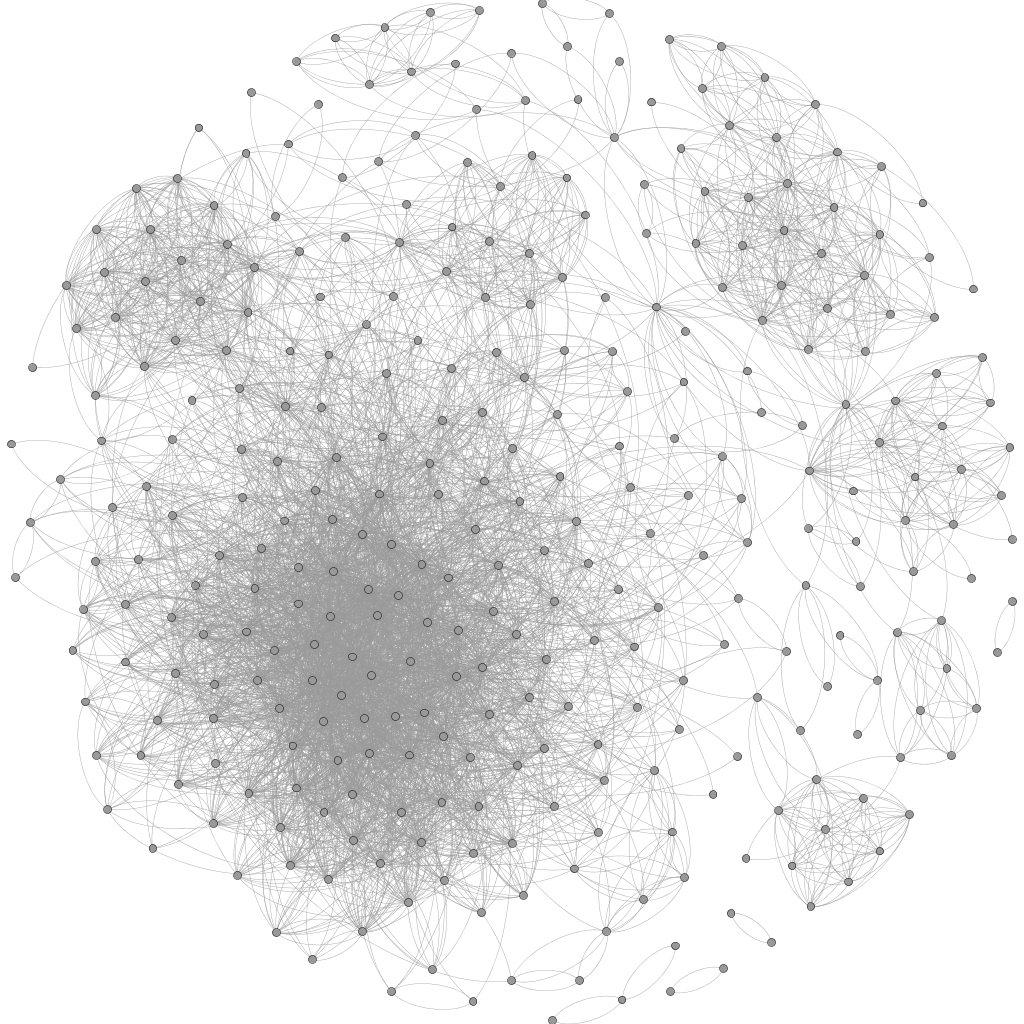
\includegraphics[scale=0.4]{fb0_graph.png}
        \end{center}
        
    \section{Results}
    
        Here is the 2D plot of graph data mapped on the plane points using {\em cmdscale} in {\em R} \cite{cmdscale}.
        
        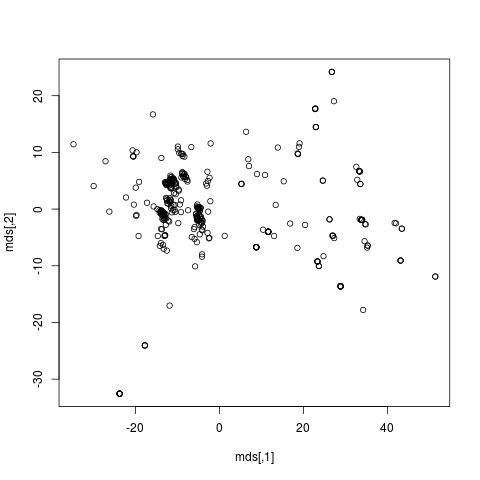
\includegraphics[scale=0.8]{fb0_2d.png}
        
        \subsection{Runtime}
        
            Here we will evaluate the runtime of the proposed {\em Dense Community Problem} with respect to the {\em brute force} implementation. This comparison will be done on random data sets of different sizes. Obviously, this will give us good estimate of the runtime when we run this on {\em graph coordinates}.
        
        \subsection{All Pair Distances}
        
            Here we will compare the variation of the distances between any two nodes in the original graph and the {\em graph coordinates}. For a good approximation the variations of the all pairwise distances in the two instances should match with each other.
            
        \subsection{Diameter}
            
            If we use the solution for the {\em Dense Community Problem} and do a binary search on the on the diameter value {\em d}, we can easily find out the diameter of the graph. The intention here is to evaluate how well we are able to estimate the diameter of the graph using {\em graph coordinates} and the {\em Dense Community Problem} algorithm. This is a way to validate our approach to get a approximate solution of the diameter.
            
    \section{Code}
    
        The code that I wrote for the project can be found on {\em Github} at \url{https://github.com/nomind/DataMiningFall2012}.
        
    \section{References}
     
        \printbibliography
    
\end{document}

